\subsection{Créer un wallet Ethereum}

\begin{frame}{Créer un wallet avec MetaMask}
  \begin{columns}
    \begin{column}{0.7\textwidth}
      \begin{itemize}
        \item Ceux qui on déjà un wallet : bonne sieste
        \item Les autres, installez l'extension MetaMask sur votre navigateur (Chrome / Firefox)
        \item Effectuez l'onboarding et notez bien la phrase de récupération
      \end{itemize}
    \end{column}
    \begin{column}{0.25\textwidth}
      \begin{figure}
        \resizebox{\textwidth}{!}{
          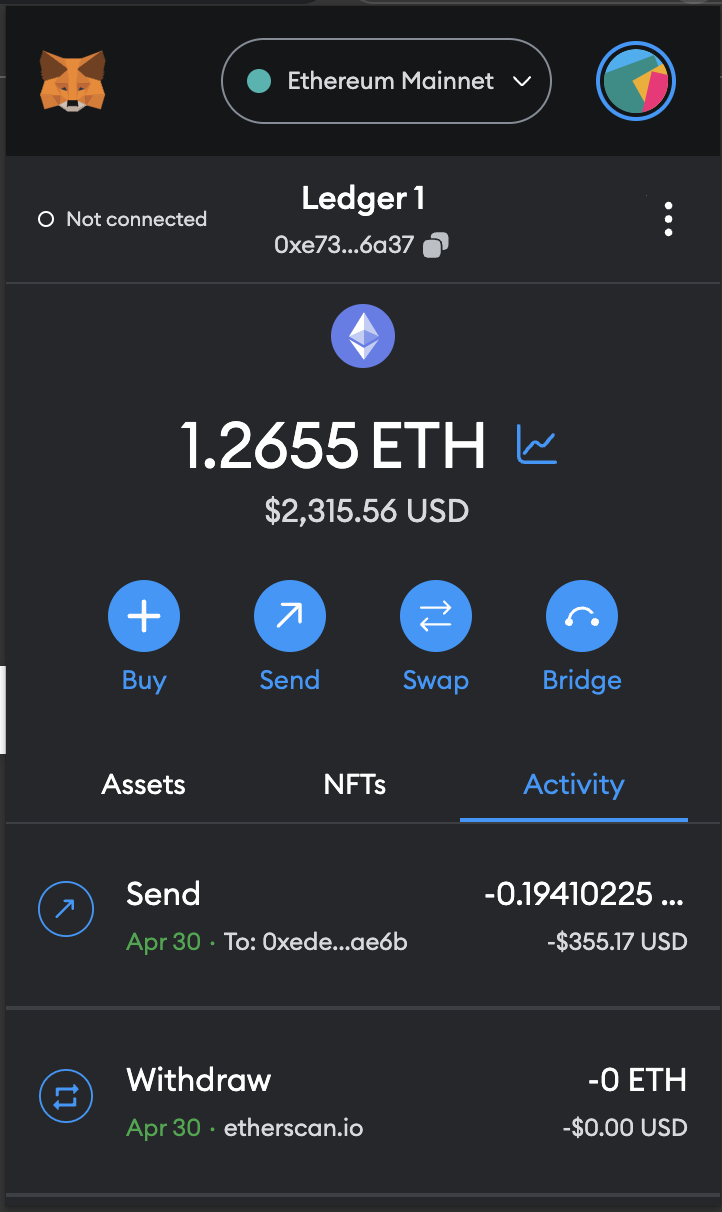
\includegraphics{img/metamask.png}
        }
      \end{figure}
    \end{column}
    \begin{column}{0.05\textwidth}\end{column}
  \end{columns}
\end{frame}

\begin{frame}{Seed phrase}
  Lors de la création d'un wallet avec MetaMask, une phrase de douze mots est générée.

  \begin{center}
    \begin{tcolorbox}[arc=1ex, colback=myuniversity, colframe=myuniversity, left=3pt, right=3pt, top=3pt, bottom=2pt]
      \vspace*{1cm}
      \begin{center}
        \begin{huge}
          \textcolor{white}{
            Il faut absolument la sauvegarder en lieu sûr.\\
            Quiconque l'obtient peut accéder à tout votre wallet, vos cryptos et vos NFTs !
          }
        \end{huge}
      \end{center}
      \vspace*{1cm}
    \end{tcolorbox}
  \end{center}
\end{frame}